
\documentclass[12pt, class=report,crop=false]{standalone}
\usepackage[screen]{../exo7book}


\begin{document}

%====================================================================
\chapitre{Calcul différentiel}
%====================================================================

% A garder
%\DeclareMathOperator{\grad}{grad}  % dans le préambule
\newcommand{\grad}{\operatorname{grad}} % dans le document


Pour une fonction de plusieurs variables,  
il y a une dérivée pour chacune des variables, qu'on appelle dérivée partielle. L'ensemble des dérivées partielles permet de 
reconstituer une approximation linéaire de la fonction : c'est la différentielle.


%%%%%%%%%%%%%%%%%%%%%%%%%%%%%%%%%%%%%%%%%%%%%%%%%%%%%
\section{Dérivées partielles}

Rappelons la notion de dérivée.
Soit $f : \Rr \to \Rr$ une fonction d'une seule variable.
La \defi{dérivée} de $f$ en $x_0 \in \Rr$, si elle existe, est : 
$$f'(x_0) = \lim_{h \to 0} \frac{f(x_0 + h) - f(x_0)}{h}.$$

\begin{exemple}
La fonction $f : \Rr \to \Rr$ définie par $f(x)=x^2$ est dérivable, de dérivée $f'(x_0)=2x_0$. En effet lorsque $h$ tend vers $0$ :
$$\frac{(x_0+h)^2-x_0^2}{h}=2x_0+h \quad \underset{h\to 0}{\longrightarrow} \quad 2x_0.$$
\end{exemple}


%----------------------------------------------------
\subsection{Définition}

\begin{definition}
Soit $f : U \subset \Rr^n \to \Rr$. 
On dit que $f$ admet une \defi{dérivée partielle} par rapport à la variable $x_i$ au point $x_0=(a_1,\dots, a_n) \in \Rr^n$, si la fonction d'une variable
$$x_i \mapsto f(a_1,\dots,x_i, a_{i+1},\ldots,a_n)$$
est dérivable au point $a_i$. Dit autrement, on définit la dérivée partielle de $f$ par rapport à $x_i$ au point $x_0=(a_1,\ldots, a_n)$ par  
$$
\lim_{h \rightarrow 0} 
\frac{f(a_1, \ldots, a_{i-1} , x_i + h, a_{i+1} , \dots , a_n) - f(a_1,\ldots, a_n)}{h}
$$ 
si cette limite existe.
\end{definition}

\bigskip

\evidence{Notation.}
Cette limite se note 
$$\frac{\partial f}{\partial x_i} (x_0)$$
C'est la dérivée partielle de $f$ par rapport à $x_i$ au point $x_0$. 
Le symbole \og{{}$\partial$\fg{} se lit \og{}d rond\fg{}.
Une autre notation est $\partial_{x_i} f(x_0)$ ou bien $f'_{x_i} (x_0)$.

Il y a donc $n$ dérivées partielles au point $x_0$ :
$$\frac{\partial f}{\partial x_1} (x_0)\qquad
\frac{\partial f}{\partial x_2} (x_0)\qquad
\ldots \qquad 
\frac{\partial f}{\partial x_n} (x_0)$$


\bigskip

Dans le cas d'une fonction de deux variables $(x,y) \mapsto f(x,y)$ on a :
\mybox{
$\displaystyle \frac{\partial f}{\partial x} (x_0,y_0) = \lim_{h \rightarrow 0}  \frac{f(x_0 + h ,y_0) - f(x_0,y_0)}{h}
\qquad
\frac{\partial f}{\partial y} (x_0,y_0) = \lim_{k \rightarrow 0}  \frac{f(x_0,y_0 + k) - f(x_0,y_0)}{k}$
}


\bigskip

\begin{remarque*}
Pour une fonction d'une variable $f : \Rr \to \Rr$,
on distingue le nombre dérivé $f'(x_0)$ et la fonction dérivée $f'$ définie par $x \mapsto f'(x)$. Il en est de même avec les dérivées partielles. Pour $f : \Rr^2 \to \Rr$
\begin{itemize}
  \item $\displaystyle \frac{\partial f}{\partial x} (x_0,y_0)$ et $\displaystyle \frac{\partial f}{\partial y} (x_0,y_0)$
  sont des nombres réels.
  
  \item $\displaystyle \frac{\partial f}{\partial x}$ et $\displaystyle \frac{\partial f}{\partial x}$ sont des fonctions de deux variables, par exemple :
$$\begin{array}{cccc}
 \dfrac{\partial f}{\partial x} : & \Rr^2 & \longrightarrow & \Rr \\
                                 & (x,y) & \longmapsto & \dfrac{\partial f}{\partial x} (x,y)
\end{array}$$
\end{itemize}
\end{remarque*}



%----------------------------------------------------
\subsection{Exemples}


\evidence{Méthode.}
Pour calculer une dérivée partielle par rapport à une variable, on n'utilise que rarement la définition avec les limites, car il suffit de dériver par rapport à cette variable en considérant les autres variables comme des constantes.


\begin{exemple}
Calculer les dérivées partielles premières de la fonction 
$f : \Rr^2 \to \Rr$ définie par 
$$f(x,y)=x^2e^{3y}$$

\bigskip
\emph{Solution.}

Pour calculer la dérivée partielle $\frac{\partial f}{\partial x}$, par rapport à $x$, on considère que $y$ est une constante et on dérive $x^2e ^{3y}$ comme si c'était une fonction de $x$ :
$$\frac{\partial f}{\partial x}(x,y) =2xe ^{3y}.$$
Pour l'autre dérivée  $\frac{\partial f}{\partial y}$, on considère que $x$ est une constante et on dérive $x^2e ^{3y}$ comme si c'était une fonction de $y$ :
$$\frac{\partial f}{\partial y}(x,y) = 3x^2e ^{3y}.$$
\end{exemple}



\begin{exemple}
Pour $f : \Rr^3 \to \Rr$ définie par $f(x,y,z)=\cos (x+y^2)e^{-z}$
alors 
$$\frac{\partial f}{\partial x}(x,y,z) = -\sin(x+y^2)e^{-z} \quad
\frac{\partial f}{\partial y}(x,y,z) = -2y\sin(x+y^2)e^{-z} \quad
\frac{\partial f}{\partial y}(x,y,z) = -\cos(x+y^2)e^{-z}$$
\end{exemple}


\begin{exemple}
Soit $f :\Rr^n \to \Rr$, définie par 
$f(x_1,\ldots,x_n) = x_1^2+x_2^2+\cdots + x_n^2$,
alors, pour $i=1,\ldots,n$ 
$$\frac{\partial f}{\partial x_i}(x_1,\ldots,x_n) = 2x_i.$$
\end{exemple}


\bigskip

Une fonction peut avoir des dérivées partielles sans être continue !
Nous allons le voir sur l'exemple suivant.
\begin{exemple}
La fonction $f : \Rr^2 \to \Rr$ suivante admet des dérivées partielles en tout point mais n'est pas continue en $(0,0)$ :
$$f(x,y) = \left \lbrace
\begin{array}{ll}
\dfrac{xy}{x^2 + y^2} & \text{ si } (x,y) \neq (0,0) \\
0 & \text{ en } (0,0)
\end{array}
\right.$$


\begin{enumerate}
  \item \textbf{Non continuité à l'origine.} 
  
   Le long du chemin $\gamma(t) = (t,t)$, pour $t\neq 0$, on a $f\big( \gamma(t) \big) = \frac{t^2}{2t^2} = \frac 12$ qui ne tend pas vers $f(0,0)=0$. Donc $f$ n'est pas continue en $(0,0)$.
  
   
   
   
  \item \textbf{Dérivées partielles en dehors de l'origine.}
  
  On se place en un point $(x_0,y_0) \neq (0,0)$. Dans un voisinage de ce point $f$ est définie par $f(x,y) = \frac{xy}{x^2 + y^2}$. 
  	La fonction $x \mapsto f(x,y_0)$ est donc continue et dérivable au voisinage de $x_0$. La dérivée partielle s'obtient en dérivant la fonction d'une variable  $x \mapsto f(x,y_0)$. Ainsi
$$\frac{\partial f}{\partial x}(x_0,y_0) = \frac{y_0^3-x_0^2y_0}{(x_0^2+y_0^2)^2}.$$  	
De même, en dérivant la fonction $y \mapsto f(x_0,y)$, on trouve 
$$\frac{\partial f}{\partial y}(x_0,y_0) = \frac{x_0^3-x_0y_0^2}{(x_0^2+y_0^2)^2}.$$  

  \item \textbf{Dérivées partielles à l'origine.}
  
  Comme la fonction $f$ est définie en $(0,0)$ par une formule spéciale, il faut revenir à la définition de ce que sont les dérivées partielles à l'aide des limites.
  
  Pour calculer $\frac{\partial f}{\partial x}(0,0)$, on calcule en $(x_0,y_0)=(0,0)$ :
  $$\frac{f(0+h,0) - f(0,0)}{h} = \frac{0}{h} = 0 \underset{h\to 0}{\longrightarrow} 0$$
  
  Donc $\frac{\partial f}{\partial x}(0,0) = 0$.
  
  De même 
   $$\frac{f(0,0+k) - f(0,0)}{k} = \frac{0}{k} = 0 \underset{k\to 0}{\longrightarrow} 0$$
  
  Donc $\frac{\partial f}{\partial y}(0,0) = 0$.  
  
  
\end{enumerate}
  
Conclusion : quelque que soit le point $(x_0,y_0)\in\Rr^2$, les dérivées partielles $\frac{\partial f}{\partial x}(x_0,y_0)$ et $\frac{\partial f}{\partial y}(x_0,y_0)$ existent.
\end{exemple}



%----------------------------------------------------
\subsection{Dérivée directionnelle}

Il est possible de généraliser la notion de dérivée partielle.
\begin{definition}
Soit $f : \Rr^n \to \Rr$.
Soit $v \in \Rr^n$ un vecteur non nul. La \defi{dérivée directionnelle} de $f$ 
en $x_0 \in \Rr^n$ suivant le vecteur $v$ est définie, si elle existe, par
$$D_{v}f(x_0)= \lim_{t\to 0} \frac{f(x_0 + t v)-f(x_0)}{t}.$$
\end{definition}


Pour une fonction $f : \Rr^2 \to \Rr$, la dérivée directionnelle au point $(x_0,y_0)$ suivant le vecteur $v=(h,k)$ est donc donnée par 
$$D_{v}f(x_0,y_0)= \lim_{t\to 0} \frac{f(x_0 + t h,y_0+tk)-f(x_0,y_0)}{t}.$$


\begin{exemple}
Soit $f$ la fonction définie sur $\Rr^2$ par
$$f(x,y)=\frac{x^3+y^3}{x^2+y^2} \quad \text{ si }(x,y)\neq (0,0)\quad \text{ et }\quad f(0,0)= 0.$$

\'Etudier l'existence de la dérivée de $f$ suivant un vecteur non nul au point $(0,0)$.


\bigskip
\emph{Solution.}

Pour tout vecteur $v=(h,k)$ non nul, on a :
$$\lim _{t\to 0}\frac{f(0+th,0+tk)-f(0,0)}{t}=
\frac{\frac{(th)^3+(tk)^3}{(th)^2+(tk)^2} - 0}{t} =
\frac{h^3+k^3}{h^2+k^2}.$$
Donc $f$ admet une dérivée suivant tout vecteur non nul au point $(0,0)$
et, lorsque $v=(h,k)$,  $D_v f (0,0) = \frac{h^3+k^3}{h^2+k^2}$.
\end{exemple}


\bigskip

De façon générale, si le vecteur $v$ est un vecteur de la base canonique, on retrouve une dérivée partielle. Soit $f : \Rr^2 \to \Rr$.
\begin{enumerate}
\item Si $v=(1,0)$, alors $D_{v}f(x,y) = \frac{\partial f}{\partial x}(x,y)$.
\item Si $v=(0,1)$, on retrouve $D_{v}f(x,y) = \frac{\partial f}{\partial y}(x,y)$.
\end{enumerate}

Lorsque $f$ est différentiable (voir plus loin dans ce chapitre) nous aurons une formule simple et directe pour calculer $D_vf(x,y)$ à partir des dérivées partielles.
Si $f$ est différentiable et $v=(h,k)$ alors
$$D_vf(x,y) = h \frac{\partial f}{\partial x}(x,y) + k \frac{\partial f}{\partial y}(x,y).$$
 

\bigskip
\evidence{Interprétation géométrique.}

Pour une fonction d'une variable, la dérivée est la pente de la tangente au graphe de la fonction (le graphe est ici une courbe). Pour une fonction de deux variables $(x,y) \mapsto f(x,y)$, les dérivées partielles indiquent les pentes au graphe de $f$ selon certaines directions (le graphe est ici une surface). Plus précisément :

\begin{itemize}
  \item $\frac{\partial f}{\partial x} (x_0,y_0)$ est la pente au graphe de $f$
 au-dessus de $(x_0,y_0)$ suivant la direction de l'axe $(Ox)$.
 En effet cette pente est celle de la tangente à la courbe $z = f(x,y_0)$ et est donnée par la dérivée de $x \mapsto f(x,y_0)$ en $x_0$. C'est donc bien $\frac{\partial f}{\partial x} (x_0,y_0)$.
 
 \item $\frac{\partial f}{\partial y} (x_0,y_0)$ est la pente au graphe de $f$
 au-dessus de $(x_0,y_0)$ suivant la direction de l'axe $(Oy)$.
 
 \item Plus généralement, si $v$ est un vecteur unitaire (i.e. de norme $1$) alors
 $D_vf(x_0,y_0)$ est la pente de la tangente, suivant la direction $v$.
\end{itemize}

 
 
\bigskip 
Sur la figure de gauche, la dérivée partielle  $\frac{\partial f}{\partial x}$ indique la pente de la tranche parallèle à l'axe $(Ox)$\couleurnb{ (en orange)}{}. Sur la figure de droite, la dérivée partielle  $\frac{\partial f}{\partial y}$ indique la pente de la tranche parallèle à l'axe $(Oy)$\couleurnb{ (en vert)}{}.


\myfigure{0.8}{
  \tikzinput{fig-calculdiff-04}
  \tikzinput{fig-calculdiff-05}
} 

Ci-dessous, la dérivée directionnelle $D_vf$ indique la pente d'une tranche \couleurnb{(en rouge)}{} dans la direction d'un vecteur $v$.

\myfigure{1.1}{
 \tikzinput{fig-calculdiff-06}
} 

\bigskip

%----------------------------------------------------
\begin{miniexercices}
\sauteligne
\begin{enumerate}
  \item En utilisant seulement la définition avec les limites, calculer les dérivées partielles de la fonction $f$, définie par $f(x,y) = x^2y$.
  
  \item Calculer les dérivées partielles de la fonction $f$ définie par  $f(x,y) = e^{xy^2}$. Mêmes questions avec $f(x,y) = x^2 + 3y^2 - 2\sin(xy)$ ; $f(x,y) = \sqrt{1 - x^2 - y^2}$ ; $f(x,y,z) = xy^2 + ze^{y/z}$ ; $f(x_1,\ldots,x_n)= x_1\ln(x_1+\cdots+x_n)$

  \item Soit $f : \Rr^2 \to \Rr$ définie par $f(x,y) = \left \lbrace
\begin{array}{cc}
0 & \text{ si }  0 < y < x^2 \\
1 & \text{ sinon}
\end{array}
\right.$.
Montrer que $f$ a des dérivées partielles en $(0,0)$, mais n'est pas continue en $(0,0)$.

  \item Soit $f : \Rr^2 \to \Rr$ définie par $f(x,y) = xy^2+x+y$. Calculer la dérivée directionnelle de $f$ en $(0,0)$ le long de tout vecteur non nul $v=(h,k)$. Pour quel vecteur $v$ unitaire, cette dérivée est-elle maximale ?
  
\end{enumerate}
\end{miniexercices}





%%%%%%%%%%%%%%%%%%%%%%%%%%%%%%%%%%%%%%%%%%%%%%%%%%%%%
\section{Différentielle}


La différentielle est une façon de regrouper toutes les dérivées partielles dans une seule fonction.

%----------------------------------------------------
\subsection{Différentiabilité}


Pour une fonction $f : \Rr \to \Rr$ d'une seule variable, une autre façon d'écrire qu'elle est dérivable en $x_0$ est qu'il existe $\ell \in \Rr$ tel que 
$$\lim_{h \rightarrow 0} \frac{f(x_0 + h) - f(x_0) - \ell \cdot h}{h} = 0$$
Et on note ce $\ell$ par $f'(x_0)$. De sorte que l'on a 
$f(x_0+h) \simeq f(x_0) + f'(x_0)\cdot h$ (pour $h$ réel, assez petit).
Autrement dit, on approche l'application $h \mapsto f(x_0+h) - f(x_0)$
par une fonction linéaire $h \mapsto f'(x_0) \cdot h$.

\bigskip

Nous allons faire ce même travail en dimension supérieure.
\begin{definition}
Soit $f : \Rr^n \to \Rr$. La fonction $f$ est \defi{différentiable} en $x_0 \in \Rr^n$, s'il existe une application linéaire $\ell : \Rr^n \to \Rr$ telle que :
$$\lim_{\|h\| \to 0}  \frac{f(x_0+ h) - f(x_0) - \ell(h)}{\|h\|} = 0$$
L'application $\ell $ est la \defi{différentielle} de $f$ en $x_0$ et se note $\dd_f(x_0)$.
\end{definition}


Dans le cas des fonction d'une variable on a $\dd_f(x_0) = f'(x_0)$ (et $\dd_f(x_0)(h) = f'(x_0)\cdot h$).
Dans le cas des fonctions de plusieurs variables, on verra juste après comment écrire la différentielle à l'aide des dérivées partielles.
Noter que $\dd_f(x_0)$ est une application de $\Rr^n$ vers $\Rr$ (comme $f$), ainsi $\dd_f(x_0)(h)$ est un réel (pour chaque $h\in\Rr^n$).


\bigskip

De même qu'en une variable, si une fonction est dérivable, alors elle est continue, on a :
\begin{proposition}
\label{prop:diffcont}
Si $f$ est différentiable en $x_0 \in \Rr^n$, alors $f$ est continue en $x_0$.
\end{proposition}

\begin{proof}
Notons $g$ la fonction définie par $g(h)=\frac{f(x_0+h) - f(x_0) - \dd_f(x_0)(h)}{\|h\|}$. Alors 
$$f(x_0 + h)=f(x_0) + \dd_f(x_0)(h) +\|h\|g(h)$$
et il est clair que $\dd_f(x_0)(h)$ et $\|h\|g(h)$ tendent vers $0$, lorsque $h$ tend vers le vecteur nul. Donc la limite de $f$ en $x_0$ existe et vaut $f(x_0)$, ainsi $f$ est continue en $x_0$.
\end{proof}

\begin{exemple}
Si $\ell : \Rr^n \to \Rr$ est linéaire, alors $\ell$ est différentiable et sa différentielle en tout point est l'application $\ell$ elle-même : pour tout $x_0 \in \Rr^n$ et $h \in \R^n$,
$$
\dd_\ell (x_0) (h) = \ell(h).
$$ 
\end{exemple}


%----------------------------------------------------
\subsection{Différentielle}


\begin{proposition}
\label{prop:differ}
Si $f : \Rr^n \to \Rr$ est différentiable en $x_0 \in \Rr^n$, alors ses dérivées partielles existent et on a :
$$
\dd_f(x_0)(h) = 
h_1 \frac{\partial f}{\partial x_1}(x_0)  + \cdots + h_n \frac{\partial f}{\partial x_n}(x_0)  
$$
où $h = (h_1,\ldots,h_n)$.
\end{proposition}
En particulier, lorsqu'elle existe, la différentielle est unique.

\bigskip

Pour $f : \Rr^2 \to \Rr$ différentiable en $(x_0,y_0)$, la formule est
\mybox{$
\dd_f(x_0,y_0)(h,k) = 
h \frac{\partial f}{\partial x}(x_0,y_0) + 
k \frac{\partial f}{\partial y}(x_0,y_0)
$}

\begin{proof}
Prouvons la formule pour deux variables.
Soit $f : \Rr^2 \to \Rr$ différentiable en $(x_0,y_0) \in \Rr^2$.
Soit $\ell(h,k) = ah + bk$ sa différentielle, ainsi
$$\frac{f(x_0+ h,y_0+k) - f(x_0,y_0) - \ell(h,k)}{\|(h,k)\|} \longrightarrow 0$$
Pour $(h,k) = (t,0)$, avec $t>0$ et $t \to 0$ on a :
$$\frac{f(x_0+ t,y_0) - f(x_0,y_0) - t\ell(1,0)}{t}
= \frac{f(x_0+ t,y_0) - f(x_0,y_0)}{t} - \ell(1,0) \longrightarrow  0$$
C'est exactement dire que 
$$\frac{\partial f}{\partial x}(x_0,y_0) = \ell(1,0) = a$$

Avec $(h,k) = (0,t)$, on prouve que 
$$\frac{\partial f}{\partial y}(x_0,y_0) = \ell(0,1) = b$$

Ainsi 
$$\ell(h,k) = h \frac{\partial f}{\partial x}(x_0,y_0) +
k \frac{\partial f}{\partial k}(x_0,y_0).$$
\end{proof}




Pour montrer qu'une fonction est différentiable, on peut utiliser que la somme, le produit, l'inverse (d'une fonction ne s'annulant pas), la composition de fonctions différentiables est différentiable. Sinon il faut revenir à la définition : 
\begin{enumerate}
  \item tout d'abord on calcule les dérivées partielles 
  $\frac{\partial f}{\partial x}(x_0,y_0)$,  $\frac{\partial f}{\partial y}(x_0,y_0)$, 
  
  \item on écrit la candidate à la différentielle $
\ell(h,k) = 
h \frac{\partial f}{\partial x}(x_0,y_0) + 
k \frac{\partial f}{\partial y}(x_0,y_0)
$,

  \item il faut enfin prouver la limite :
$$\frac{f(x_0+ h,y_0+k) - f(x_0,y_0) - \ell(h,k)}{\|(h,k)\|} \longrightarrow  0.$$
  
\end{enumerate}




\begin{exemple}
\'Etudier la différentiabilité en tout point de la fonction $f$ définie par
$$f(x,y)= x-3y + \frac{x^4}{x^2+y^2}\quad\mbox{ si }(x,y)\neq (0,0)\qquad \text{ et }\quad f(0,0)=0.$$

 
\bigskip
\emph{Solution.}

\begin{itemize}
  \item En dehors de $(0,0)$ la fonction $f$ est différentiable, car $f$ est une somme, produit, inverse de fonctions différentiables (car $x^2+y^2$ ne s'annule qu'à l'origine).
  
  \item En $(0,0)$ il faut étudier la différentiabilité à la main.
  \begin{itemize}
    \item Dérivée partielle en $x$ :
      
  $$\frac{\partial f}{\partial x}(0,0) = \lim _{h\to 0}\frac{f(h,0)-f(0,0)}{h}=\lim _{h\to 0}\frac{h+h^2}{h}=1$$
  
    
    \item Dérivée partielle en $y$ :
      
  $$\frac{\partial f}{\partial y}(0,0) = \lim _{k\to 0}\frac{f(0,k)-f(0,0)}{k}=\lim_{k\to 0}\frac{-3k}{k}=-3$$
    
    \item Le candidat à être la différentielle est
$$\ell(h,k) = 
h \frac{\partial f}{\partial x}(0,0) + 
k \frac{\partial f}{\partial y}(0,0)
= h-3k$$

    \item On calcule :
$$0 \le \frac{f(0+h,0+k) - f(0,0) - \ell(h,k)}{\sqrt{h^2+k^2}}
=  \frac{h^4}{(h^2+k^2)^{\frac{3}{2}}}
\le \frac{h^4}{|h|^3}
=|h|
\underset{(h,k)\to(0,0)}{\longrightarrow} 0
.$$    
    
  \end{itemize}
    
Donc $f$ est différentiable au point $(0,0)$ et $\dd_f (0,0)(h,k) = h-3k$.
  
\end{itemize}

\end{exemple}

%----------------------------------------------------
\subsection{Lien avec les dérivées partielles}


\bigskip
\evidence{Dérivées partielles.}

On a vu dans la proposition \ref{prop:differ} que, si $f : \Rr^2 \to \Rr$ est différentiable en $(x_0,y_0)$, alors
$$\dd_f (x_0,y_0) (1,0) = \frac{\partial f}{\partial x}(x_0,y_0)
\qquad \text{ et } \qquad
\dd_f (x_0,y_0) (0,1) = \frac{\partial f}{\partial y}(x_0,y_0)$$

En toute dimension, pour $f : \Rr^n \to \Rr$ différentiable en $x_0 \in \Rr^n$, et $e_i$ le $i$-ème vecteur de la base canonique :
$$\dd_f (x_0) (e_i) = \frac{\partial f}{\partial x_i}(x_0)$$



\bigskip
\evidence{Dérivée directionnelle.}

Plus généralement, si $f : \Rr^n \to \Rr$ est différentiable en $x_0 \in \Rr^n$, alors $\dd_f (x_0) (v) = D_v f(x_0)$.
Pour $f : \Rr^2 \to \Rr$ cela signifie que si $v=(h,k)$, alors :
\mybox{$D_{(h,k)} f(x_0,y_0) = h \frac{\partial f}{\partial x}(x_0,y_0) +
k \frac{\partial f}{\partial k}(x_0,y_0).$}

Si $f$ n'est pas différentiable, cette formule peut être fausse.

\bigskip
\evidence{Gradient.}

Le gradient est une autre façon de coder la différentielle.
Le \defi{gradient} de $f$ en $x_0$ est le vecteur :
$$\grad f (x_0) =
\begin{pmatrix}
\dfrac{\partial f}{\partial x_{1}} (x_0)\\
\vdots \\
\dfrac{\partial f}{\partial x_n}(x_0)
\end{pmatrix}.$$

Si $f$ est différentiable en $x_0$, alors
$$\dd_f (x_0) (v) = \langle \grad f (x_0) \mid v \rangle.$$
où $\langle u \mid v \rangle$ est le produit scalaire de $u$ et $v$.

Nous reviendrons en détails sur le gradient et ses applications dans le chapitre \og{}Gradient et théorème des accroissements finis\fg{}.


\bigskip
\evidence{Résumé.}

Lorsque $f$ est différentiable alors la différentielle, la dérivée directionnelle, et le gradient encode la même information et sont reliés  
par les formules :
\mybox{$\displaystyle
D_v f(x_0) = \dd_f (x_0) (v) = \langle \grad f (x_0) \mid v \rangle.
$}



\begin{exemple}
Soit $f : \Rr^2 \to \Rr$ définie par 
$$f(x,y) =  \ln(1+x+y^2).$$

\begin{enumerate}
  \item Calculer les dérivées partielles de $f$.
  \item Montrer que $f$ est différentiable.
  \item Calculer la gradient de $f$ en $(0,1)$.
  \item Calculer la dérivée directionnelle de $f$ en $(0,1)$ le long du vecteur $(2,1)$.
\end{enumerate}
 
\bigskip
\emph{Solution.}


Tout d'abord $f$ est définie sur $U = \big\{ (x,y) \in \Rr^2 \mid 1+x+y^2>0 \big\}$.

\myfigure{1}{
  \tikzinput{fig-calculdiff-02}
}


\begin{enumerate}
  \item Les dérivées partielles sont :
  $$\frac{\partial f}{\partial x}(x,y) = \frac{1}{1+x+y^2} \qquad\qquad
  \frac{\partial f}{\partial y}(x,y) = \frac{2y}{1+x+y^2}$$
  
  
  \item $f$ est différentiable sur $U$ comme somme, produit, inverse d'une fonction ne s'annulant pas et composition de fonctions différentiables.
  
  \item Le gradient s'obtient directement à partir des dérivées partielles :
  $$\grad f (0,1) = \begin{pmatrix} \dfrac{\partial f}{\partial x}(0,1) \\\dfrac{\partial f}{\partial y}(0,1) \end{pmatrix} = 
\begin{pmatrix} \frac12 \\ 1 \end{pmatrix}$$
  
  \item Comme $f$ est différentiable, la dérivée directionnelle est simplement la combinaison linéaire des dérivées partielles :
  $$D_{(2,1)} f(0,1) = 2\times \frac{\partial f}{\partial x}(0,1)+1\times
  \frac{\partial f}{\partial y}(0,1) = 2$$
\end{enumerate} 
  
\end{exemple}



%----------------------------------------------------
\begin{miniexercices}
\sauteligne
\begin{enumerate}
  \item Soit $g : \Rr \to \Rr$ dérivable. Soit $f : \Rr^2 \to \Rr$ définie par $f(x,y)= g(x+y)$. Montrer que $f$ est différentiable et que
  $\dd_f (x_0,y_0)(h,k) = g'(x_0+y_0)h + g'(x_0+y_0)k$.
  
  \item Soit $f(x,y) = 2xy-7x+8y$. En utilisant la définition, montrer que $f$ est différentiable et calculer sa différentielle.
  
  \item Soit $f$ définie par $f(x,y) = ye^{x/y}$. Trouver le domaine de définition de $f$. Montrer que $f$ est différentiable. Calculer les dérivées partielles. Calculer la dérivée directionnelle en $(4,2)$ selon le vecteur $v = (-1,1)$.
  
\end{enumerate}
\end{miniexercices}





%%%%%%%%%%%%%%%%%%%%%%%%%%%%%%%%%%%%%%%%%%%%%%%%%%%%%
\section{Fonction $\mathcal{C}^1$}

Dans la pratique les fonctions seront souvent de classe $\mathcal{C}^1$, ce qui implique différentiable, et est plus facile à vérifier. 


%----------------------------------------------------
\subsection{Définition}

\begin{definition}
Soit $f: \Rr^n \to \Rr$. On dit que $f$ est de classe $\mathcal{C}^1$ si les dérivées partielles $\frac{\partial f}{\partial x_i}$
existent et sont continues.
\end{definition}

On peut bien sûr limiter la définition à un ouvert. Par exemple, soit $U$ un ouvert de $\Rr^2$, $f : U\subset \Rr^2 \to \Rr$, sera de classe $\mathcal{C}^1$ sur $U$ si $\frac{\partial f}{\partial x}$ et $\frac{\partial f}{\partial y}$ existent et sont continues sur $U$.


\begin{theoreme}
\label{th:foncc1}
Si $f$ est de classe $\mathcal{C}^1$, alors $f$ est différentiable.
\end{theoreme}

Une autre façon de dire que $f$ est différentiable est de dire que $f$ admet un \defi{développement limité à l'ordre $1$}. Pour $f : \Rr^2 \to \Rr$
au point $(x_0,y_0)$, si $f$ est différentiable alors
$$f(x_0+h,y_0+k)=f(x_0,y_0)+h\frac{\partial f}{\partial x}(x_0,y_0)+k\frac{\partial f}{\partial y}(x_0,y_0)+o\left(\|(h,k)\|\right).$$

\bigskip

On rappelle la notation \og{}petit o\fg{}.

\textbf{Notation.} Soit $g :\Rr^2\to \Rr$ une fonction définie au voisinage de $(0,0)$. On dit que $g$ est \defi{négligeable} par rapport à $\|(x,y)\|^n$ au voisinage de $(0,0)$ et on note $g=o\left(\|(x,y)\|^n\right)$ si 
$$\lim_{(x,y)\to(0,0)}\frac{g(x,y)}{\|(x,y)\|^n}=0.$$

\begin{exemple}
Soit $f : \Rr^2 \to \Rr$ définie par $f(x,y)=\sin x e ^{2y}$.

\begin{itemize}
  \item On a : $\frac{\partial f}{\partial x}(x,y)=\cos x e ^{2y}$ et $\frac{\partial f}{\partial y}(x,y)=2\sin x e ^{2y}$. Les deux dérivées partielles existent et sont continues donc $f$ est de classe $\mathcal{C}^1$ sur tout $\Rr^2$. 
  
  \item En particulier $f$ est différentiable en tout point $(x_0,y_0) \in \Rr^2$ et 
  $$\dd_f (x_0,y_0)(h,k) = h\cos x_0 e ^{2y_0}+k2\sin x_0 e ^{2y_0}$$
  
  \item Par exemple, pour $(x_0,y_0) = (\frac\pi6,1)$, on a le développement limité :
  $$f(\tfrac\pi6+h,1+k) = f(\tfrac\pi6,1) + 
  h\frac{\partial f}{\partial x}(\tfrac\pi6,1)+
  k \frac{\partial f}{\partial y}(\tfrac\pi6,1) + o\left(\|(h,k)\|\right)$$
  Ce qui donne :
 $$f(\tfrac\pi6+h,1+k) = \frac{1}{2}e^2 + \frac{\sqrt3}{2}e^2h + 
 e^2k + \epsilon(h,k)\sqrt{h^2+k^2}$$
 où $\epsilon(h,k) \to 0$ lorsque $(h,k) \to (0,0)$. 
\end{itemize}

\end{exemple}



\begin{proof}
Soit $f$ une fonction $\mathcal{C}^1$ au voisinage du point $(x_0,y_0)$ : elle admet donc des dérivées partielles continues au voisinage de $(x_0,y_0)$. 


Pour $(h,k)\in \Rr^2$, on a :
$$f(x_0+h,y_0+k)-f(x_0,y_0)=\big[f(x_0+h,y_0)-f(x_0,y_0)\big]
+\big[f(x_0+h,y_0+k)-f(x_0+h,y_0)\big].$$

Les fonctions $x\mapsto f(x,y_0)$ et $y\mapsto f(x_0+h,y)$ sont dérivables respectivement aux points $x_0$ et $y_0$. Donc
$$f(x_0+h,y_0)-f(x_0,y_0)=h\frac{\partial f}{\partial x}(x_0,y_0)+o(h)$$
et
$$f(x_0+h,y_0+k)-f(x_0+h,y_0)=k\frac{\partial f}{\partial y}(x_0+h,y_0)+o(k).$$
Or, $\frac{\partial f}{\partial y}$ est continue au point $(x_0,y_0)$, donc $\frac{\partial f}{\partial y}(x_0+h,y_0)=\frac{\partial f}{\partial y}(x_0y_0)+o(1)$. D'où
$$f(x_0+h,y_0+k)-f(x_0,y_0)=h\frac{\partial f}{\partial x}(x_0,y_0)+k\frac{\partial f}{\partial x}(x_0,y_0)+h\epsilon _1(h)+k\epsilon _2(k)$$
avec $\lim _{h\to 0}\epsilon _1(h)=0=\lim _{k\to 0}\epsilon _2(k)$. Or
$$\frac{|h\epsilon _1(h)+k\epsilon _2(k)|}{\|(h,k)\|}\le |\epsilon _1(h)|+|\epsilon _2(k)| \underset{(h,k)\to(0,0)}{\longrightarrow} 0.$$
Donc
$$f(x_0+h,y_0+k)-f(x_0,y_0)=\dd_f (x_0,y_0)(h,k)+o\left(\|(h,k)\|\right).$$
Ainsi $f$ admet un développement limité d'ordre $1$ au point $(x_0,y_0)$, autrement dit $f$ est différentiable en ce point.
\end{proof}



%----------------------------------------------------
\subsection{Résumé}
 

\myfigure{1}{
  \tikzinput{fig-calculdiff-01}
}

\begin{itemize}
  \item Les équivalences sont issues des définitions.
  \item Les implications viennent du théorème \ref{th:foncc1}, de la proposition \ref{prop:diffcont} et de la proposition \ref{prop:differ}.
  \item Les implications inverses sont fausses : voir les exemples ci-dessous.
\end{itemize}
    
 

%----------------------------------------------------
\subsection{Contre-exemples}


Dans cette partie on justifie que les énoncés précédents ne peuvent pas être améliorés. Cette section peut être passée en première lecture.


\bigskip


Si $f$ est différentiable, alors $f$ est continue. La réciproque est fausse, comme le prouve l'exemple suivant.

\begin{exemple}
Soit $f : \Rr^2 \to \Rr$ définie par $f(x,y) = |x+y|$.
Alors $f$ est continue (comme somme et composée de fonctions continues), mais n'est pas différentiable. Par exemple $\frac{\partial f}{\partial x}$ n'est pas définie en $(0,0)$, car 
$$\frac{f(0+h,0)-f(0,0)}{h} = \frac{|h|}{h}$$
n'a pas de limite lorsque $h \to 0$. (Plus précisément c'est $+1$, pour les $h>0$ et $-1$ pour les $h<0$). Donc $f$ n'est pas différentiable en $(0,0)$.


\begin{center}
  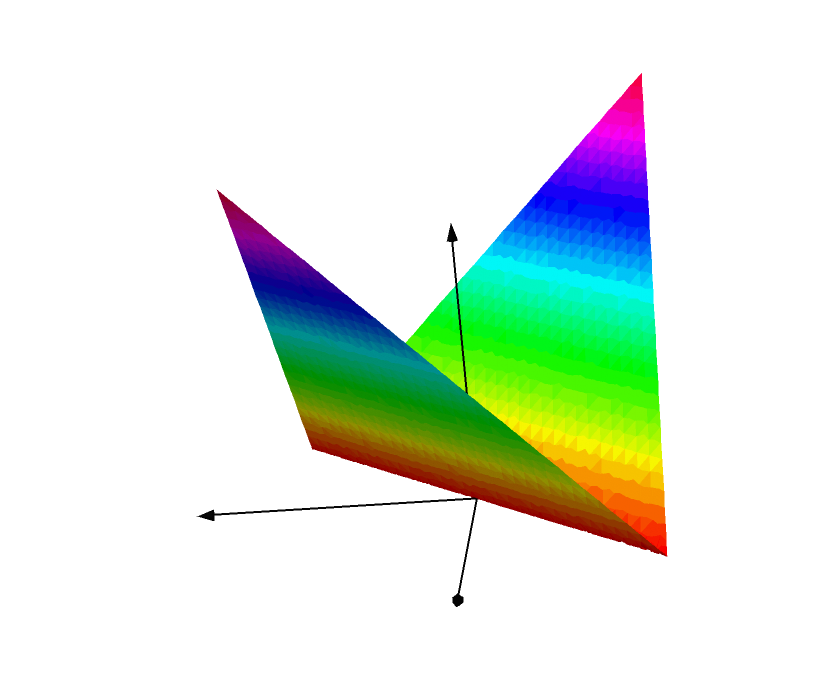
\includegraphics[scale=0.3]{figures/fig-calculdiff-03}
\end{center}


Sur la figure du graphe de $f$, on devine que, en tout point de la droite $(y=-x)$, $f$ n'est pas différentiable.
\end{exemple}


\bigskip



Si $f$ est différentiable, alors $f$ admet des dérivées partielles et des dérivées directionnelles dans toutes les directions. La réciproque est fausse, comme le prouve l'exemple suivant.

\begin{exemple}
Soit $f:\Rr^2\to \Rr$ la fonction définie par
$$f(x,y)=\frac{y^3}{\sqrt{x^2+y^4}}\quad \text{ si }(x,y)\neq (0,0)\qquad \text{ et }\quad f(0,0)=0.$$
Montrer que $f$ admet une dérivée suivant tout vecteur non nul au point $(0,0)$, mais qu'elle n'y est pas différentiable.


\bigskip
\emph{Solution.}

\begin{enumerate}
\item Soit $v=(h,k)\neq (0,0)$.
\begin{itemize}
  \item Si $h=0$, on a $\displaystyle \frac{f(t \cdot v)-f(0,0)}{t}=\frac{f(0,tk)}{t}=k$.
  \item Si $h\neq 0$, on a $\displaystyle \left\vert \frac{f(t\cdot v)-f(0,0)}{t}\right\vert= \left\vert \frac{k^3t^2}{\sqrt{h^2t^2+h^4t^4}}\right\vert \le \left\vert \frac{k^3}{h}\right\vert |t|\underset{t\to 0}{\longrightarrow} 0$.
\end{itemize}
Ainsi $\displaystyle D_{v}f(0,0)=
\left\{
\begin{array}{ccc}
k&\text{ si }& h =0 \\ 
0&\text{ si }& h\neq 0. 
\end{array}\right.$


\item Avec $v=(1,0)$, on aura $\frac{\partial f}{\partial x}(0,0)=0$, avec $v=(0,1)$, on aura $\frac{\partial f}{\partial y}(0,0)=1$. 
Le candidat à être la différentielle en $(0,0)$ est donc $\ell(h,k)  = k$.
Mais l'expression
$$\epsilon (h,k)=\frac{f(h,k)-f(0,0)-\ell(h,k)}{\sqrt{h^2+k^2}}=\frac{k^3-k\sqrt{h^2+k^4}}{\sqrt{h^2+k^2}\sqrt{h^2+k^4}},$$
ne tend pas vers $0$ car $\lim _{t\to 0^+}\epsilon (t,t)=-\frac{1}{\sqrt{2}}$. Donc $f$ n'est pas différentiable au point $(0,0)$.
\end{enumerate}
\end{exemple}

\bigskip

Si $f$ est de classe $\mathcal{C}^1$, alors elle différentiable. La réciproque est fausse, comme le prouve l'exemple suivant.

\begin{exemple}
Soit $f:\Rr^2\to \Rr$ telle que
$$f(x,y)=y^2\sin \frac{1}{x^2+y^2}\quad \text{ si }(x,y)\neq (0,0)\qquad \text{ et }\quad f(0,0)=0.$$
Montrer que $f$ est différentiable en tout point de $\Rr^2$ sans être de classe $\mathscr{C}^1$ à l'origine.

\bigskip
\emph{Solution.}


\begin{itemize}
  \item \textbf{En dehors de l'origine.}
  
Les dérivées partielles 
$$\frac{\partial f}{\partial x}(x,y)=-\frac{2xy^2}{(x^2+y^2)^2}\cos \frac{1}{x^2+y^2}$$
et
$$\frac{\partial f}{\partial y}(x,y)=2y\sin \frac{1}{x^2+y^2}-\frac{2y^3}{(x^2+y^2)^2}\cos \frac{1}{x^2+y^2}$$
existent et sont continues sur $\Rr^2\setminus \{(0,0)\}$. 
Ainsi $f$ est de classe $\mathscr{C}^1$ sur $\Rr^2\setminus \{(0,0)\}$ et, par le théorème \ref{th:foncc1}, est donc différentiable sur $\Rr^2\setminus \{(0,0)\}$.


  \item \textbf{Différentiabilité au point $(0,0)$.} 
  \begin{itemize}
    \item Calculons les dérivées partielles de $f$ au point $(0,0)$. Comme $f(x,0)=0$ alors 
$$\frac{\partial f}{\partial x}(0,0)=\lim _{h\to 0}\frac{f(h,0)-f(0,0)}{h}=0.$$
et comme $f(0,y) = y^2\sin \frac{1}{y^2}$ alors 
$$\frac{\partial f}{\partial y}(0,0) = \lim _{k\to 0}\frac{f(0,k)-f(0,0)}{k}=\lim _{k\to 0}k\sin \frac{1}{k^2}=0$$
  \item Le candidat à la différentielle en $(0,0)$ est donc $\ell(h,k) = 0$. 
  \item De plus
$$\lim _{(h,k)\to (0,0)}\frac{f(h,k)-f(0,0)-\ell(h,k)}{\sqrt{h^2+k^2}}=\lim _{(h,k)\to (0,0)}\frac{k^2}{\sqrt{h^2+k^2}}\sin \frac{1}{h^2+k^2}.$$
Or, $\displaystyle \left|\frac{k^2}{\sqrt{h^2+k^2}}\sin \frac{1}{h^2+k^2}\right|\le |k|\underset{(h,k)\to(0,0)}{\longrightarrow 0}$. Donc $f$ est différentiable au point $(0,0)$.
  \end{itemize}
  \item \textbf{Conclusion.} 
  
  La fonction $f$ est différentiable sur $\Rr^2$. Par ailleurs, 
$$\frac{\partial f}{\partial x}(t,t)=-\frac{1}{2t}\cos \frac{1}{2t^2}$$ n'a pas de limite lorsque $t\to0$. La dérivée partielle n'est donc pas continue en $(0,0)$. Ainsi $f$ n'est pas de classe $\mathcal{C}^1$ à l'origine.

\end{itemize}
\end{exemple}



%----------------------------------------------------
\begin{miniexercices}
\sauteligne
\begin{enumerate}
  \item Justifier que la fonction définie par 
  $f(x,y) =  \ln(1+x+2y)\cos(y)$ est différentiable sur son ensemble de définition. \'Ecrire le développement limité à l'ordre $1$ de $f$ en $(0,0)$. Même travail avec $f(x,y) = \sqrt{1+x-2y}$.

  \item Montrer que la fonction
$f(x,y) = \left \lbrace
\begin{array}{ll}
\frac{x^3}{x^2 + y^2} & \text{ si } (x,y) \neq (0,0) \\
0 & \text{ en } (0,0)
\end{array}
\right.$
admet des dérivées partielles en tout point, mais n'est pas différentiable en $(0,0)$.


  \item Montrer que la fonction de deux variables
$f(x,y) = \left \lbrace
\begin{array}{ll}
x^2\sin \frac{1}{x} & \text{ si } x \neq 0 \\
0 & \text{ sinon }
\end{array}
\right.$
 est différentiable, mais que $\frac{\partial f}{\partial x}$ n'est pas continue en $(0,0)$.
 
\end{enumerate}
\end{miniexercices}

\auteurs{
\\
D'après des cours de Abdellah Hanani (Lille), 
Goulwen Fichou et Stéphane Leborgne (Rennes),
Laurent Pujo-Menjouet (Lyon). 

Revu et augmenté par Arnaud Bodin.

Relu par Barbara Tumpach et [...].%Stéphanie Bodin et Vianney Combet.
}


\finchapitre 
\end{document}


